% Copyright (c) 2014,2016 Casper Ti. Vector
% Public domain.

\chapter{CAPS设计与实现} \label{chap:design}
\section{CAPS综述}
随着处理器中的核数越来越多,共享缓存的竞争问题也愈发严重。目前,还没有一个可以在真实系统上可以运行的缓存优化框架,我们希望通过我们的努力实现这样一个框架的原型。我们称之为CAPS,它可以满足以下几个方面的要求:(1)\textbf{可以在真实系统中运行};(2)\textbf{实现细粒度分配控制};(3)\textbf{具有良好的可扩展性,在核数较多时依然有很好的适应性};(4)\textbf{具备灵活性,支持多种优化策略}。

共享缓存分配优化的步骤一般包含以下三个过程:
\begin{enumerate}
\item 预测过程(Prediction)。首先需要在任意分配情况下,对每个并发程序的性能进行预测和评估。性能参数包括失效率(Miss Rate)和周期指令数(IPC)等等。预测的指标用来为后面的决策提供参考依据。
\item 决策过程(Decision-making)。根据预测的指标和优化目标,做出一个分配决策,给出优化分配方案。针对不同的优化目标,可能会采取不同的策略和算法。
\item 执行过程(Enforcement)。通过某种技术实施优化分配分配方案,让分配真正产生作用。
\end{enumerate}

若要在真实系统上实施分配,CAT技术是目前唯一的方法。所以CAPS必须倚仗于CAT作为执行分配方案的技术。而采用哪样的分配技术对前两个步骤,即预测和决策过程,又有深远的影响,因为决策所得到的分配必须符合分配技术的要求,而预测又是为决策提供服务。如上一章所述,CAT技术要求分配必须连续,有限的可分配路数的情况下,要实现细粒度、可扩展和灵活的划分是非常困难的。然而,CAT允许分配之间重叠的这一特性却带来很大的操作空间。虽然在分配重叠,尤其是部分重叠,会给预测模型和分配决策带来了更大的挑战,但是我们通过研究探索,在CAPS中实现了一个全新的预测模型,以及一个基于模拟退火的决策算法,可以支持部分重叠下的CAT分配的性能预测和优化决策,让上述提出的四点目标得以满足。

CAPS框架的整体架构如图\ref{fig:caps_overview}所示。首先,需要对并发工作负载中的每个程序进行一次离线采样分析,分析得到该程序的缓存特征,包括缓存失效率曲线(MRC),以及访存频率(API)。离线采样分析只需要进行一次即可,结果被保存在硬盘中以便之后使用。CAPS最重要的两个模块是预测模型和优化算法。预测模块可以对任意CAT分配下,包括部分重叠的分配方案,对每个程序的性能进行预测。预测指标包括缓存失效率(Miss Rate)和周期指令数(IPC)。优化算法依赖于预测模块,它通过模拟退火算法,在CAT分配方案的解空间中进行启发式搜索,对于每个可行解调用预测模块进行预测,再根据预测结果找到一个最优分配方案。最后,通过CAT技术实施这一方案。

\begin{figure}[htbp] 
    \centering
    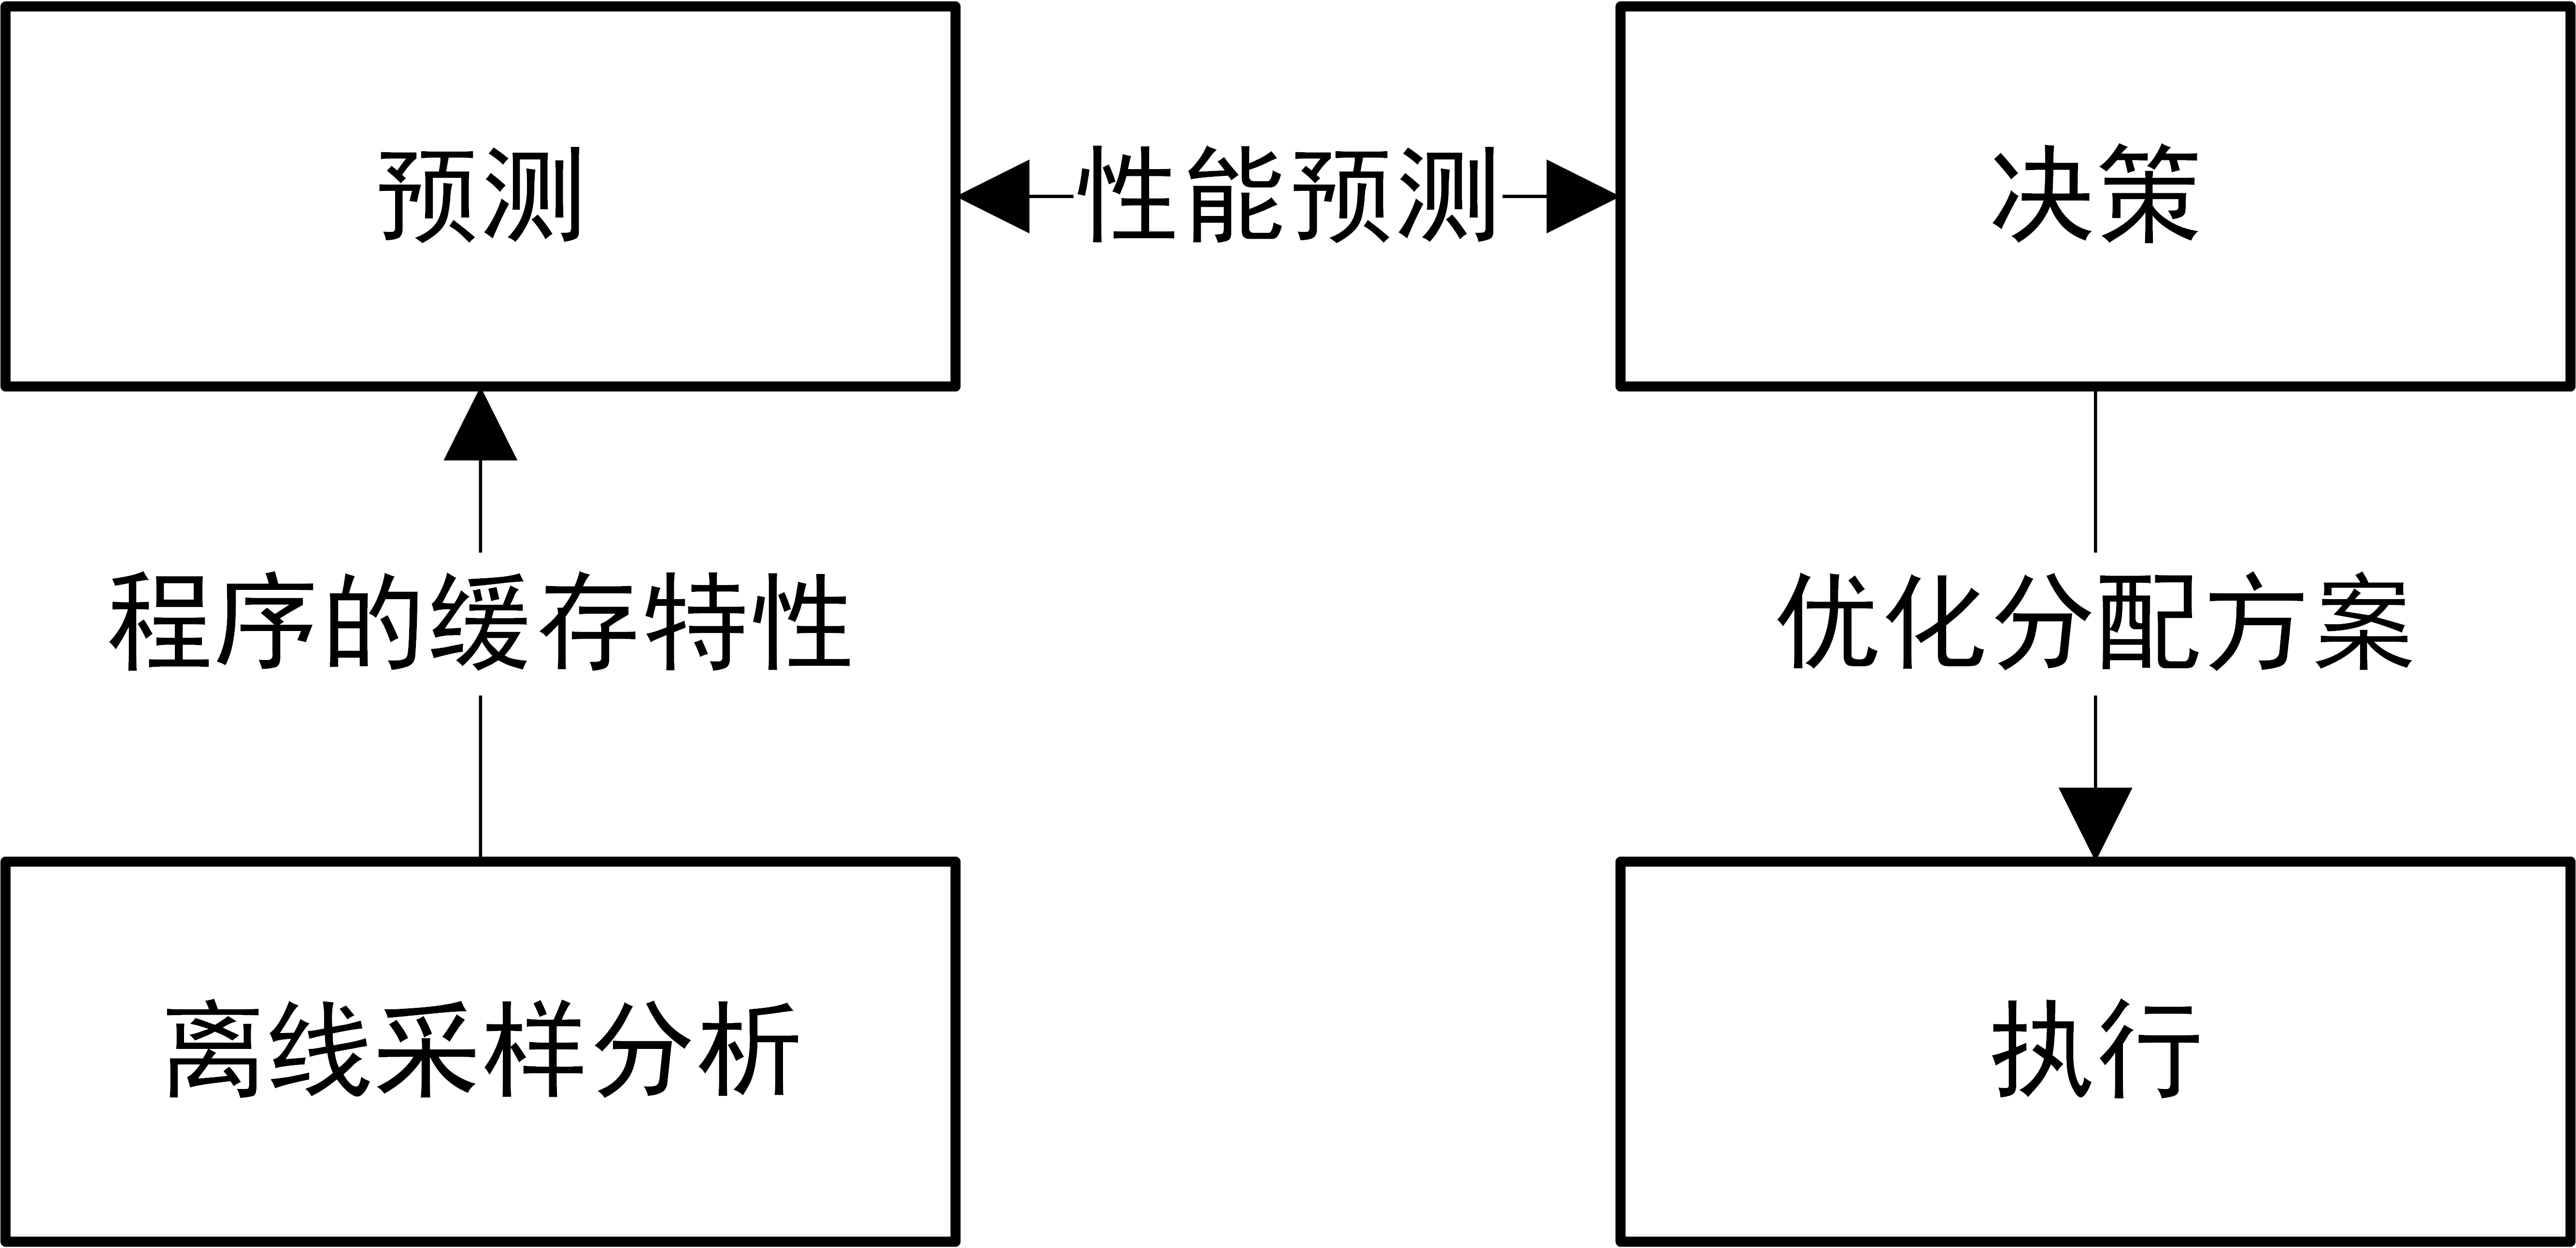
\includegraphics[width=0.6\linewidth]{figures/caps_overview.png}
    \caption{CAPS架构}
    \label{fig:caps_overview}
\end{figure}

CAPS框架两个最重要的模块是预测模型和优化算法。在给定一个优化目标后,预测模块与优化模块两者相互协作,在较短时间内可以生成一个优化分配方案。同时CAPS还具有良好的可扩展性,支持多种多样的优化目标。我们在本文中实现了5种优化指标及相应的策略,这些目标分别侧重性能、公平性以及服务质量(QoS)等不同的方面。经过我们在真机上的实验评估,无论在哪个优化指标下,CAPS都能起到良好的优化效果。

\section{预测模型} \label{sec:prediction}
\subsection{模型概述}
在本章中,我们将介绍CAPS的预测模型。对缓存失效率的预测是优化的基础,它的准确性会直接影响到整个优化框架的效果。由于优化决策依赖于预测模型提供的信息,不准确的预测结果可能会导致错误的分配决策。虽然前人对失效率预测进行了大量工作,但它们都不适用于CAT下的预测,因为前人的研究都没有考虑过分配间部分重叠的情况。为了应对部分重叠的问题,我们为CAPS推导了一个全新的预测模型。

CAPS预测模型可以较为准确地预测出,多个并发执行的程序在任意CAT分配下,每个程序的缓存失效率(Miss Rate)和周期指令数(IPC)。一个CAT分配包括每个线程/核的分配(CLOS)的集合。CAPS预测模型的输入包括每个并发程序的失效率曲线(Miss Rate Curve,MRC)和访存指令占比(Accesses per Instruction, API),以及加载于它们身上的CAT分配。MRC和API可以描绘出一个程序的局部性和缓存访问频率等特征,这两个指标都可以通过离线采样分析得到,在第\ref{sec:prediction_sample}节中会详细介绍。MRC刻画了失效率随缓存大小变化的情况,它是描述某个程序的缓存敏感度的一种有效手段。MRC是这样一条曲线,它的横轴是缓存占用,纵轴是失效率。API用来刻画程序的访存频率,它代表了程序对缓存的污染程度,通常访存频率越高,在与别的程序竞争中越有优势。

CAT技术规定,一个程序的分配可与一个或多个其他程序的分配重叠。重叠的部分就意味着有不止一个程序会竞争使用这一缓存区域。对于独占的缓存区域,程序的缓存占用就是分配的大小,而对于共享区域,每个程序实际占用的缓存大小就不是一目了然了。预测的关键问题就在于弄清楚这些重叠部分的竞争结果,即程序在竞争下实际得到的缓存大小。我们通过一个迭代算法解决了这一问题,算法会在第\ref{sec:prediction_iteration}节中详细阐述,简而言之,该算法通过迭代过程找到均衡状态时每个程序的实际占用,每次迭代相当于一小段程序执行周期,在这个过程中,它们的缓存占用发生了改变。我们假设每个程序的访存模式都是稳定的,所以在均衡状态下,各个程序的缓存占用也会达到稳定,这个稳定值就是我们要求的答案。根据真实占用和MRC很容易推导出每个程序的失效率,再根据失效率估计出IPC,就得到了模型的输出。值得一提的是,实际中每个程序的访存模式都会随着运行阶段的变化而变化,CAPS预测模型也可以适应于这种变化,但是需要实时地获取MRC。在本文中,我们只关注程序的平均性能,所以只使用离线采样的平均MRC和API作为输入。

在我们对4到15个程序的工作负载进行了多达750次实验,结果表明CAPS预测模型具有较高的预测准确率,同时还能保持较低的额外开销,具体的实验评估见第\ref{chap:evaluation}章。


\subsection{离线采样分析} \label{sec:prediction_sample}
本节中,我们将介绍如何通过PIN这一工具离线采样得到程序的MRC和API。研究者们对于如何获取MRC进行了大量的研究,在CAPS中,我们借鉴了基于平均淘汰时间(Average Eviction Time,AET)的技术~\parencite{hu2016kinect}。任何MRC采样技术都需要程序的访存序列,它是构建MRC的基础。在本文中,我们使用PIN~\parencite{luk2005pin}这一工具对访存序列进行追踪。

Pin是一款针对x86 指令系统的二进制代码分析工具(Binary Instrumentation Tool)。它能够在不改变原有程序执行逻辑的前提下,在该程序的任何指令前后插入用户自定义的代码片段。Pin 包含引擎(PinEngine)和工具(PinTools)两个部分。PinEngine是一个不开源的可执行程序,是其核心部分,它负责完成二进制代码解析和改写。PinTools是由用户自己编写的一些函数库,定义了代码替换的具体规则、以及要插入的代码片段。当Pin执行时,PinTools 会以模块的形式被动态链接到PinEngine中,二者协同完成整个代码替换。

Pin与AET结合构建MRC的工作流程如下:
\begin{enumerate}
\item 被测试的基准程序作为输入被Pin引擎读入翻译缓存,PinEngine对它的二进制代码进行静态分析,标记出函数、基本块等;
\item 完成一批代码分析后,PinEngine会自动调用PinTools中注册的代码替换回调函数(Instrumentation Callback)。该函数根据用户自己的需要,扫描Pin分析出来的指令流,再调用PinEngine提供的代码替换接口,将自定义的指令回调函数(Execution Callback)插入到程序的指令流中。本例中,我们在所有访存指令之前加入了自己的代码memop(ip, ea);
\item PinEngine将修改后的代码片段载入其执行缓存,并跳转执行它。
\item 执行到访存指令时,修改后的代码片段自动调用先前插入的指令回调函数memop(),且PinEngine会计算出该指令的指令指针ip和被访问的内存地址ea,作为参数传递给回调函数。回调函数memop()的行为非常简单,它将内存地址ea这个参数以二进制的方式写入Memory Trace文件中。
\item 当被测试的基准程序执行完毕或执行到指定时间后,将Memory Trace文件作为输入AET模型进行失效率曲线MRC构建。
\item AET模型计算完毕后,输出失效率曲线MRC。
\end{enumerate}

\begin{figure}[htbp] 
    \centering
    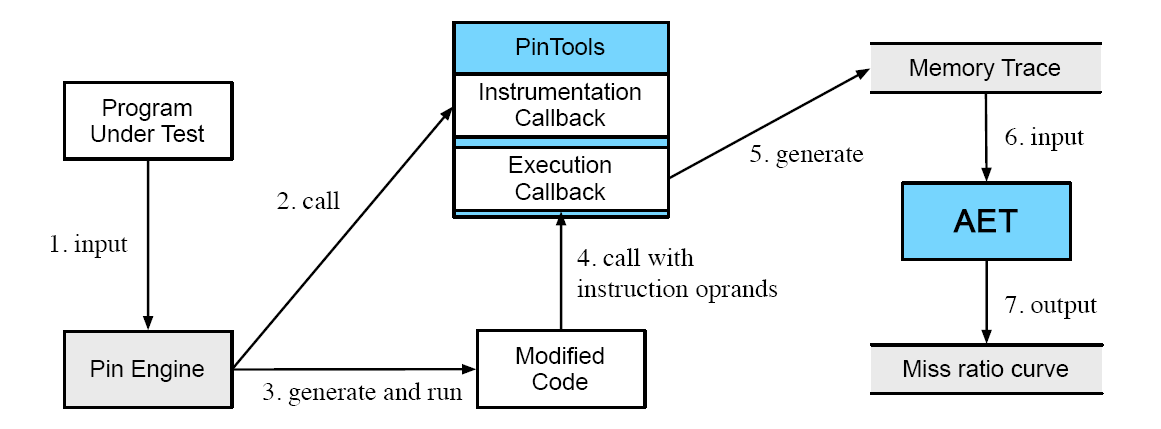
\includegraphics[width=0.8\linewidth]{figures/pin.png}
    \caption{利用Pin和AET构建MRC的流程图}
    \label{fig:pin}
\end{figure}

AET是一个先进的MRC采样技术,它可以在较低的时间空间开销下根据访存序列得到一个准确的MRC。虽然额外开销对于离线优化框架来说并没有那么重要,但我们仍然想控制时空开销,因为我们计划在未来将CAPS拓展到在线环境中。AET具有线性的时间复杂度,并且可以通过随机采样来减少运行时间,同时也能保持较高的MRC准确率。

以往的MRC技术多是基于重用距离,它被定义为对同一数据的相邻两次访问间所间隔的不同数据数。通过构造出重用距离直方图,然后累加得到MRC。但是完整地统计出重用距离直方图会带来巨大的时间和空间开销。从渐进意义上来说,对于$N$个读写访问到$M$个不同的地址,构造重用距离直方图的时间复杂度为$O(N\log M)$,空间复杂度为$O(M)$~\parencite{olken1981efficient}。

基于AET的方法引入了平均淘汰时间(Average Eviction Time,AET)这一概念。失效时间(Eviction Time)被定义为最近一次访问到失效所经历的时间。LRU缓存可以被看作是一个栈,栈中数据按最近访问时间排序。最近访问多的在栈顶,最近访问少的在栈底。栈底被挤出去的就是被替换掉了。AET实际上就是缓存块从栈顶移动到栈底并出栈的平均时间。AET模型的输入是重用时间而不是重用距离,两者的差别在于,前者并不需要统计两次重用之间不同的访问次数,只需要统计总次数,所以可以通过随机采样的方式大大减少时间和空间消耗,因为只要采样的重用时间分布与真实的分布一样,AET一样可以得到准确的MRC。通过随机采样一小部分的访存,大量的时间和空间开销可以被节省下来。然而,对于部分共享的情况,只有MRC是不够的,下一节我们将介绍如何通过一个迭代算法来求解重叠情况下的预测问题。

% 在步骤6 中,计算重用距离需要知道与上次访问该地址之间间隔的不同地址的
% 数目。这需要用一个散列表记住所有访问过的内存地址,然后用链表将它们串起,
% 在软件中模拟LRU 队列的行为。由于程序的访存操作数以百亿计,优化这一算法
% 是十分必要的。本文采用了文献[56]中提到的树算法来加速重用距离的近似计算。

\subsection{迭代预测算法} \label{sec:prediction_iteration}


在分配没有重叠的情况下,系统给定的分配大小就是该程序缓存占用的的实际大小,根据MRC就可以直接得到失效率。然而,在分配重叠的情况下,问题就变得复杂了。有一些研究针对完全重叠的情况进行预测~\parencite{chandra2005predicting, suh2014analytical, xiang2011all, xiang2011linear, hu2016kinect}。但是,这些研究对于我们所面对问题,即部分重叠分配的预测,都无能为力。简单地把部分重叠分配下的每个完全重叠片段看成是一个自由竞争的小缓存块是不正确的。因为CAT是通过缓存失效来驱动的,在CAT下,如果是一个缓存命中,那么它可以命中在LLC的任何地方,即使是在这个核的分配之外,此时CAT不发挥作用。CAT只在缓存失效时才发生作用,CAT限制了该缓存失效只能替换掉分配区域内的一个缓存块。所以,对于处理器核来说,它发出的访问请求并不是均匀分布在它的分配中,而是它引起的失效均匀分布到它的分配中。因此,我们不能把每个重叠的缓存片段当成一个独立的完全共享的缓存,所以之前很多对于完全共享缓存的研究不能套用到部分共享的情况下来。

为了解决部分共享下失效率的预测问题,我们推导了一个全新的模型,通过一个迭代算法来预测部分共享缓存的情况下各个程序的缓存占用和失效率。首先,我们根据每个分配的起点和终点,将整个缓存空间划分成多个缓存片段。每个缓存片段是一个完全重叠子区域,它们组合在一起构成整个LLC。图\ref{fig:interval}展示了这个分段方法的示例,可以看到,该示例中有三个线程分别被分配了各自的缓存区域,根据分配的起点和终点,该缓存空间被划分成了5个片段,每个片段都是一个独占或完全重叠的子区域。

\begin{figure}[htbp] 
    \centering
    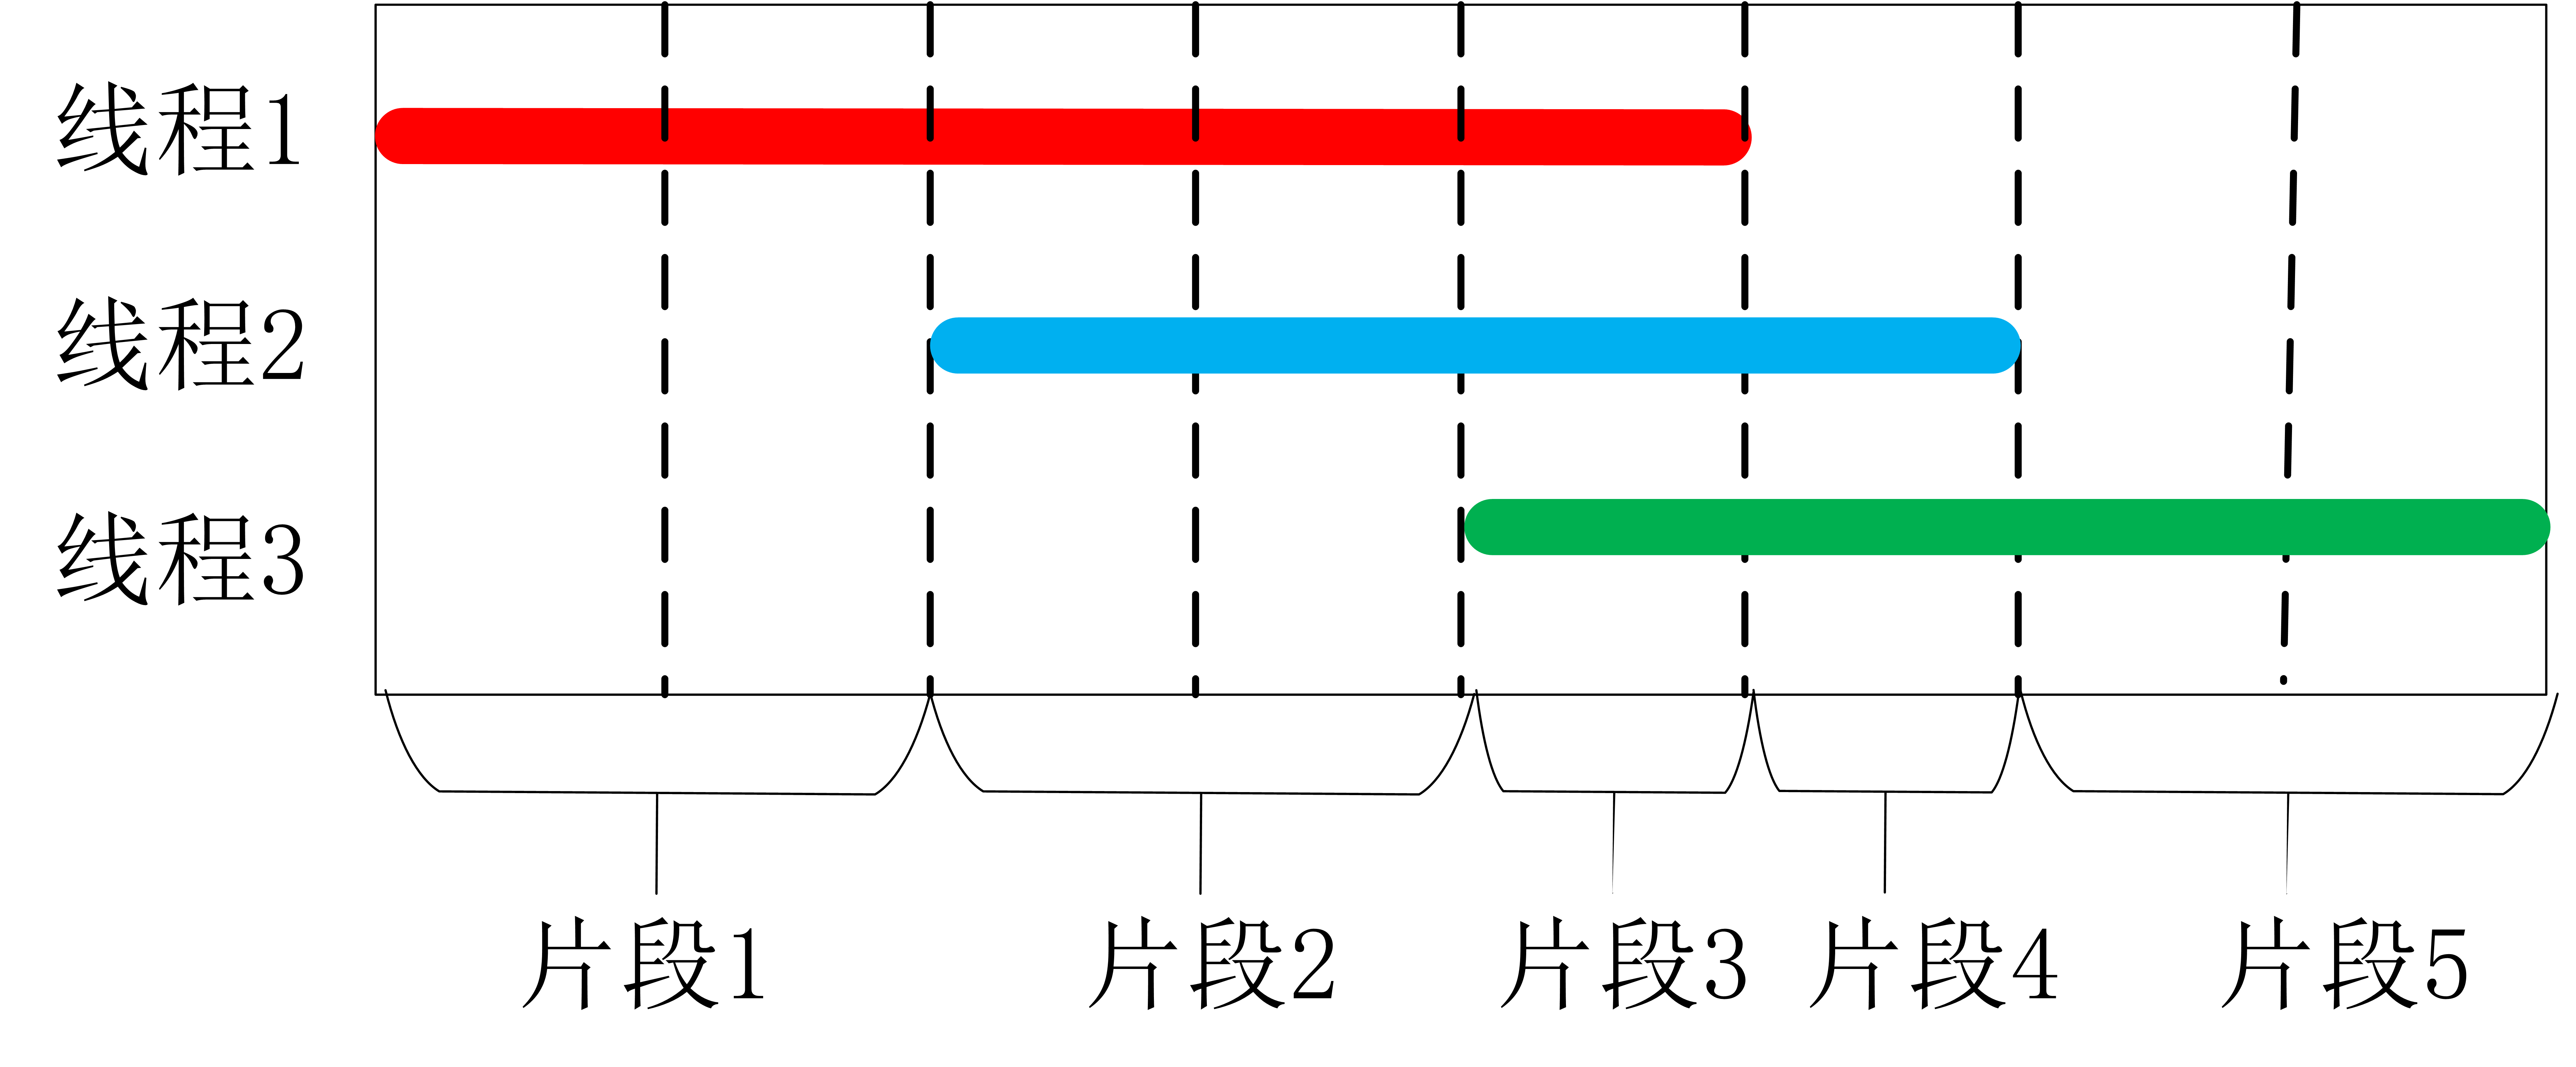
\includegraphics[width=0.8\linewidth]{figures/interval.png}
    \caption{缓存分段示意图}
    \label{fig:interval}
\end{figure}

分段过后,一个程序的分配区域可以被看成几个连续的缓存片段的组合。显然,无论在何种分配组合下,总的缓存片段数都会小于等于总的缓存路数。在每个缓存片段中,分配中包含这段的程序之间互相竞争,我们预测算法的核心就在于预测每个缓存片段的竞争结果。只要得到了每个缓存片段中各个程序的实际缓存占用,我们就可以汇总得到程序总的缓存占用,再通过MRC曲线就可以得到该程序的失效率。

在竞争中,缓存占用和失效数息息相关,竞争的深层原因实际上就是缓存失效淘汰了别的程序所占用的缓存块从而占为己有。失效数与缓存占用存在着一种负反馈的关系。失效数越多,往往意味着更多的缓存占用;反过来看,更多的缓存占用意味着更少的失效。在负反馈关系下,最后会达到一个稳定的状态,这个状态下的失效数和缓存占用都会稳定下来。假设程序的访存模式是恒定的,这个稳定状态就是程序运行时长期保持的状态,稳定状态时的缓存占用和失效率就是真实的缓存占用和失效率。CAPS预测模型的核心就是通过一个迭代算法求解这个稳定状态,算法伪代码如算法\ref{alg:pred}所示。

\begin{algorithm}
\caption{预测算法伪代码}
\label{alg:pred}
\begin{algorithmic}[1]
\renewcommand{\algorithmicforall}{\textbf{foreach}}
\renewcommand{\algorithmicrequire}{\textbf{Input:}}
\renewcommand{\algorithmicensure}{\textbf{Output:}}
\REQUIRE $MRC[i][]$ and $API[i]$ of each program $i$; a CAT scheme
\ENSURE $MissRate[i]$, $IPC[i]$ for each program $i$
\STATE Partition cache space to shared intervals based on allocations' starting and finishing points
\STATE Initialize $occupancy[i][j]$ for program $i$ in interval $j$ = (size of interval $j$) / (number of programs sharing the interval)
\WHILE {aggregate change of occupancies > threshold}
	\STATE {/* occupancy to miss rate */}
    \FORALL {program $i$}
    	\STATE $occ$ = $0$
    	\FORALL {interval $j$}
			\STATE $occ$ += $occupancy[i][j]$
        \ENDFOR
        \STATE $MissRate[i]$ = $MRC[i][occ]$
        \STATE $IPC[i]$ = $1 / (CPI_{base} + MissRate[i] * API[i] * MissPenalty)$
        \STATE $Miss[i]$ = $MissRate[i] * API[i] * IPC[i] * step$
    \ENDFOR
    \STATE {/* miss rate to occupancy */}
    \FORALL {interval $j$}
    	\STATE $TotalIntervalMiss$ = $0$
   		\FORALL {program $i$ in interval $j$}
        	\STATE $IntervalMiss[i][j]$ = $Miss[i] * IntervalSize[j] / AllocationSize[i]$
            \STATE $TotalIntervalMiss$ += $IntervalMiss[i][j]$ 
		\ENDFOR
        
        \FORALL {program $i$ in interval $j$}
        	\STATE $occupancy[i][j]$ =  $occupancy[i][j] + IntervalMiss[i][j] * (IntervalSize[j] - occupancy[i][j]) / IntervalSize[j] - (TotalIntervalMiss - IntervalMiss[i][j]) * occupancy[i][j] / IntervalSize[j]$
		\ENDFOR
    \ENDFOR
    \IF {$step$ > $minStep$}
    	\STATE $step$ = $step * StepReductionRatio$
    \ENDIF
\ENDWHILE

\STATE \textbf{return} $MissRate[]$, $IPC[]$

\end{algorithmic}
\end{algorithm}

每个程序的失效率曲线(MRC)和访存指令占比(API)是该预测算法的输入参数,该算法通过迭代过程得到稳定状态下的实际缓存占用。作为迭代的初始状态,我们首先需要给出一个初始占用。这个占用可以是随机的,并不影响最后的结果,但是会影响迭代收敛的速度。在CAPS的实现中,我们使用平均分配作为初始占用。在每次迭代的前半部分,我们根据当前的占用结果计算得到每个程序的失效率、失效数和IPC;在迭代的后半部分,我们根据当前的失效数和IPC推导出下一阶段的占用。直到缓存占用的变化程度小于一定的阈值,我们认为迭代收敛,此时的占用即是我们要求的稳定状态下的真实占用。

在介绍之前,我们引入了一个迭代步长参数$Step$来控制收敛过程。$Step$模拟在冷启动中每次迭代的步长,它也可以被看成公式\ref{eq:accesses}中的周期数。更大的步长通常意味着更快的收敛速度,但是同时也可能造成某次迭代越过了均衡点,导致迭代在均衡点两侧跳动从而无法收敛。另一方面,较小的步长可能会影响收敛速度,降低预测算法的效率。在CAPS中,我们选择了一个较大的初始$Step$,然后逐渐地降低它,每轮迭代降低5\%,直到设定的最低点。这样的话,我们可以在保证收敛到均衡点的同时提升了收敛速度。

首先我们来看迭代的前半部分,即通过当前的缓存占用来推导失效率、失效数和IPC。事实上,上一节的离线采样我们已经得到了每个程序的$MRC$,根据当前的缓存占用直接查阅MRC就可以得到失效率$MissRate$。失效数和IPC可以通过以下两个公式推导:

\begin{equation}
Misses = MissRate \times API \times IPC \times Step 
\label{eq:accesses}
\end{equation}

\begin{equation}
IPC = \frac{1}{CPI_{base} + API \times MissRate \times MissPenalty}
\label{eq:IPC}
\end{equation}

有了$MissRate$可以根据公式\ref{eq:accesses}计算得到失效数$Misses$。而$IPC$比较难以估计,因为很多因素都可以影响到IPC。这里,我们通过公式\ref{eq:IPC}来做一个近似估计。$CPI_{base}$和$MissPenalty$通过真实机器上的实验来估计。$CPI_{base}$通过一个失效率很低的测试程序来估计,而$MissPenalty$通过LLC的失效延迟来估计。   

注意,公式\ref{eq:accesses}得到的是该程序总的失效数。因为英特尔处理器使用了特殊的哈希函数来处理内存地址到缓存块的映射,可以近似地认为这种映射方式是充满了随机性的,所以缓存失效可以近似地被认为在分配区域内均匀分布。某个缓存片段中产生的失效占总体失效数的比例与片段大小占总的分配大小的比例是相同的。根据总的失效数和缓存片段大小占该程序分配区域的比例,就可以就可以得到每个缓存段的失效数。

我们再来看迭代的后半部分,即通过当前的失效数和IPC,来推导并更新缓存的占用情况。考虑到每个缓存片段的大小和竞争的程序都是不同的,对于每个缓存片段,我们分个击破。那么如何根据失效数和IPC来推导新的缓存占用呢?West等在一篇论文中介绍了一种双线程下缓存占用实时预测的方法\parencite{west2010online},该研究是通过硬件实时抓取到失效率来预测两个线程的缓存占用情况。虽然使用场景与我们的场景并不相同,但这个研究启发了我们建立了一个类似的定理用来计算多个程序的缓存占用。为了简化模型,我们假设所有程序都是单线程的,且在不同的核上执行。

\textbf{定理:}\emph{考虑一个容量为$C$的LLC,被$N$个并发程序所共享。每个程序目前分别占用了$C_1, C_2, ... , C_N$的缓存大小,并且在这一阶段分别产生了$M_1, M_2, ... , M_N$个失效。设$M$为失效数的总和,则对于程序$i$来说,它更新后的缓存占用为:$C_i' = C_i + \frac{C-C_i}{C} \cdot M_i - \frac{C_i}{C} \cdot (M-M_i)$.}

\textbf{证明:}首先,我们假设整个LLC空间已经被这$N$个程序充满。事实上,除了冷启动外,绝大多数时间LLC都是被充满的。充满状态下,每一次的失效都会淘汰一个缓存块。这时,如下公式成立:

\begin{equation}
C = \sum_{i=0}^{N} C_i
\label{eq:sumc}
\end{equation}

其次,我们假设每个缓存块都有均等的概率被替换。虽然在LRU策略下,这个假设通常是不正确的。失效的访存会替换掉最近最少被使用(LRU)的那个缓存块,这就意味着经常被访问的缓存块被替换的概率较小。然而,为了模型简洁性,我们仍然使用这一假设。事实上,这一假设不会给准确率带来很大影响\parencite{west2010online}。

当程序$i$发生了一个失效时,它淘汰掉的缓存块属于其他程序的概率为:$\frac{C-C_i}{C}$,这就相当于把缓存块从其他程序那里抢夺过来。程序$i$在单位时间内总共产生了$M_i$个失效,所以因为失效而抢夺过来的缓存块数量为:$\frac{C-C_i}{C} \cdot M_i $。在另一方面,其他程序的失效也可能从它这里抢夺一部分缓存块。一个缓存块属于程序$i$的概率为$\frac{C_i}{C}$,其他程序产生的失效数为$(M-M_i)$,所以其他程序从它这里抢夺的缓存块数量为:$\frac{C_i}{C} \cdot (M-M_i)$。在这个阶段过后,该程序占用的缓存块数量变动即为,抢夺来的缓存块减去被抢夺走的缓存块:

\begin{equation}
 \Delta C = \frac{C-C_i}{C} \cdot M_i - \frac{C_i}{C} \cdot (M-M_i)
 \label{eq:deltac}
\end{equation}

更新后的缓存占用为:

\begin{equation}
 C_i' = C_i + \frac{C-C_i}{C} \cdot M_i - \frac{C_i}{C} \cdot (M-M_i)
 \label{eq:occupancy}
\end{equation}

更新后的缓存占用仍然符合公式\ref{eq:sumc},所有$C_i'$之和仍然为$C$。在CAPS预测模型中,我们对于某个缓存片段,使用公式\ref{eq:occupancy}计算每轮迭代更新后的缓存占用,然后将所有缓存段的占用加总,就得到了该程序在当前迭代轮的总缓存占用。

此时就完成了一轮迭代,然后进入下一轮迭代的前半部分,根据更新后的缓存占用再来计算新的失效率、失效数和IPC。当缓存占用的变化率小于一定的阈值后,我们认为迭代已经收敛,即我们要求的稳定状态已经达到,CAPS预测模块会输出此时每个程序的失效率和IPC。

\section{分配优化} \label{sec:allocation}
% Copyright (c) 2014,2016 Casper Ti. Vector
% Public domain.

\subsection{算法综述}

本章节中,我们将介绍CAPS的优化算法。该优化算法基于上一章节的预测模型,可以针对一个优化目标,在较短时间内生成一个优化CAT分配方案。同时,该算法还支持不同的优化目标,我们在CAPS中实现了五个优化策略,在后文中会着重阐述。

缓存的优化问题可以被概括为一句话:给定一个优化目标,找到一个最优分配。但是在CAT技术下的优化问题将面临更大的挑战,之前的研究不用考虑部分重叠和分配位置,但CAT下的分配优化无法绕过这两点。相比于之前只考虑分配数额的优化问题,CAT优化问题的搜索空间更加庞大。之前的优化算法只需要决定每个线程需要被分配多少缓存空间,而CAT下需要决定每个分配是从哪到哪,而且还允许部分重叠。显然,搜索整个解空间显然是不现实的,搜索的时间和空间开销都是极其惊人的。可以证明,在这种情况下找到一个最优分配是一个NP-hard问题。

因此,我们的算法并不寻求一个全局绝对最优的分配方案,而只需要一个较优解。事实上,由于预测的准确率并不十分精确,所以一个全局上的绝对最优解并没有太大意义,反而在短时间内找到一个较优解有更大的意义。为此,我们从经典的模拟退火算法中吸取智慧,构建了一个基于“模拟退火”的优化算法。我们的实验表明该算法在任何优化目标下都能起到良好的效果,具体实验评估结果见第\ref{chap:evaluation}章。

\subsection{优化目标} \label{sec:opt_goals}

在介绍优化算法之前,我们先来讨论一下优化的目标。优化的目标是一个优化策略锚定的指标,是驱动一个优化算法的重要动力。一个优化指标是对系统的总体优化目标的一个量化,不同的指标侧重点也不同,总体来说可以被概括为三个方面:性能(Performance)、公平(Fairness)和服务质量(QoS)。当然,一个指标也可以兼顾两个方面,但同时兼顾三个方面是不现实的~\parencite{hsu2006communist}。优化策略的目标就是将锚定的指标最小化或最大化,同时该指标也用来在实验中评估策略的有效性。

前人的研究中提出了许多指标来抽象多个并发程序的整体效能。这些指标大多依赖于IPC和失效率这两个参数,这也是CAPS预测模型会输出这两个参数的原因。我们希望我们的优化策略具有灵活性,可以很容易适应多个指标,而不用对不同的指标设计截然不同的策略。事实上,因为预测模型预测出了失效率和IPC,只要是基于这两个参数的指标,我们的优化策略都可以直接适配。在本文中,我们选择实现了五个指标作为参考。这五个指标涵盖了各种场合下的优化需求,包括上述所说的性能、公平和服务质量这三个方面。

我们在CAPS中实现的五个指标为:

\begin{itemize}

\item \textbf{平均失效数(Average MPKI):}平均失效数Average MPKI代表平均每1000条指令的失效数(Misses Per 1000 Instructions, MPKI)。MPKI是系统评估中的常用指标之一,平均失效数代表所有并发程序的平均MPKI,它可以体现出该并发系统的缓存利用效率。较小的平均失效数意味着较高的缓存利用效率,所以针对该指标的优化策略目的就是让平均MPKI尽可能的小。另一方面,LLC缓存失效就意味着该访存指令需要访问内存,所以最小化MPKI也意味着降低内存总线的竞争。在下述公式中,我们定义$MissRate_i$为程序$i$在和别的程序并发执行时的失效率,$APKI_i$是程序$i$每1000条指令的访存指令数。Average MPKI是一个越小越好的指标。

\begin{equation}
AverageMPKI = \sum ( MissRate_i \times APKI_i ) / \#program
\label{eq:mn}
\end{equation}
	
\item \textbf{吞吐量(Throughput):}吞吐量Throughput被定义为所有程序的IPC之和,这也是一个被广泛使用的指标。针对该指标的策略力求让系统整体的IPC吞吐量最大化。它把所有并发程序看成一个整体,使得整个系统的执行效率最高。但是,该指标可能会对一些本身IPC就比较低的程序不太公平,因为降低它们的IPC并不会对整体系统的IPC之和产生非常大的影响。在下述公式中,我们定义$IPC_i$为程序$i$在并发负载中的IPC。Throughput是一个越大越好的指标。

\begin{equation}
	Throughput = \sum IPC_i
	\label{eq:IPCsum}
\end{equation}

\item \textbf{平均效率下降(Average Slowdown):}平均效率下降Average Slowdown代表着在平均情况下,程序的在共享LLC与独占LLC的执行时间之比。因为相比于一个程序独占LLC,共享的情况下或多或少都会受到一定的性能损失,所以每个程序的Slowdown一定是大于1的,平均Slowdown自然也大于1。我们定义对于程序$i$来说,它的Slowdown为$SingleIPC_i/IPC_i$,这里$SingleIPC_i$指的是当它单独运行使用全部LLC时每周期执行的指令数(IPC),$IPC_i$是在多程序并发负载中的IPC。平均Slowdown的概念与前人研究中多次提到的另一个指标,加权效率提升(Weighted Speedup),有很大相似之处~\parencite{snavely2000symbiotic,qureshi2006utility}。Weighted Speedup把并发执行的程序看成一个整体,Speedup是Slowdown的倒数,用来加总的Speedup而不是平均意义上的Slowdown,可以概括系统作为一个整体因为并发带来的效率提升。但是我们认为,每个并发的程序还可以看作独立的个体,每个程序执行各自不同的任务,这样的话针对单个程序的Slowdown可以更好地反映出程序的执行效率。相比于独占LLC,共享情况下的性能必定会下降,所以一定会引起每个程序或多或少的效率下降,换句话说每个并发程序的Slowdown一定大于1。我们把所有程序的Slowdown做算术平均,就可以得到该并发负载因为共享LLC导致的整体性能下降。Average Slowdown是一个越低越好的指标。

\begin{equation}
	AverageSlowdown = \sum\frac{SingleIPC_i}{IPC_i} / \#program
\end{equation}

\item \textbf{公平效率下降(Fair Slowdown):}公平效率下降指标Fair Slowdown兼顾了整体性能和公平性。这个指标借鉴了多个前人的研究经验~\parencite{luo2001balancing, chang2014cooperative}。如果只考虑公平性而无视性能是没有意义的,因为大家效率都很差的话,即使再公平也意义不大。我希望通过指标能在提升性能的基础上兼顾公平。与上一个指标Average Slowdown不同之处在于,本指标被定义为各个程序Slowdown的调和平均。调和平均鼓励大家的差距尽量小,鼓励各个程序的Slowdown得到均匀地改善。Fair Slowdown是一个越小越好的指标。

\begin{equation}
	FairSlowdown = \#program / {\sum\frac{IPC_i}{SingleIPC_i}}
\end{equation}

\item \textbf{最大效率下降(Maximum Slowdown):}最大效率下降Maximum Slowdown指的是所有并发程序中Slowdown最大的那一个,它兼顾了性能与服务质量(QoS)。事实上,QoS是比较难以被量化的,因为判断哪些程序优先级较高,哪些程序优先级较低本身就比较主观。在本文中,我们不讨论程序间优先级不同这一主观因素,我们把并发负载看成一个木桶,把QoS定义成木桶中最短的那块短板,也就是Slowdown最高的那个程序。这种表达QoS的方法也被之前的研究者所使用~\parencite{manikantan2012probabilistic}。Maximum Slowdown是一个越小越好的指标。

\begin{equation}
MaxSlowdown=\max(\frac{SingleIPC_i}{IPC_i})
\label{eq:qos}
\end{equation}

\end{itemize}

\subsection{优化算法}

在本节中,我们将介绍CAPS生成优化分配的算法。一个CAT分配组合包含对每一个核/线程的分配所构成的集合,一个分配是LLC中任意一段连续的路。我们的目标是找到一个优化分配,使得给定的优化指标最大或最小化。之前研究面对的分配问题只需要决定分配的数量,而CAT下由于要求分配是连续的且允许部分重叠,所以分配的位置也需要被考虑进去。

CAT下的优化算法主要存在两点挑战:

首先,搜索空间随着核数增加而呈指数级增长,当核数较多时解空间会变得极其巨大。举例来说,对于一个20路的LLC,一共有210(1+2+3+..+20)种CLOS,或者说是可能的分配情况。对于一个$N$核的工作负载,$N$个程序并发执行,那么一共可能的CAT分配数为$210^N$。在4核情况下,解空间的规模就已经达到了1,944,810,000,全部搜索一遍显然是不太现实的,甚至搜索一小部分都要耗费大量的时间。

其次,之前的优化方案都不能适用于CAT。为了避免搜索的时间消耗,之前的解决方案多是通过启发式算法来找到优化分配,例如贪心算法~\parencite{suh2004dynamic}、前瞻算法(Lookahead Algorithm)~\parencite{qureshi2006utility}等。但这些解决方案都有一个隐含的假设,就是一个缓存路只能分配给一个核,并不能被两个或多个核所共用。这个假设在它们的分配技术下是成立的,然而在CAT下并不成立。所以这些解决方案都不能直接套用在CAT上。

因此,我们需要一个全新的算法来解决CAT下的分配优化问题。我们从经典算法中吸取经验,设计了一个基于模拟退火(Simulated Annealing)的算法,它可以针对任意优化目标生成一个优化分配方案。模拟退火算法是一个随机化算法,它可以在一个庞大的解空间中找到一个全局近似最优解~\parencite{aarts1988simulated,hwang1988simulated}。该算法适合被应用在搜索空间较大并且离散的情况下,CAT优化问题的搜索空间正符合这一特征。同时,模拟退火适合在有限时间内找到一个近似最优解,而不是全局最优解。在CAT优化问题中,短时间内找一个优化解确实比花费大量时间找到一个全局绝对最优解有更大的意义。综上,模拟退火算法是CAT优化问题的一个有效的解决思路。

\begin{algorithm}
\caption{优化算法伪代码}
\label{alg:opt}
\begin{algorithmic}[1]
\renewcommand{\algorithmicforall}{\textbf{foreach}}
\renewcommand{\algorithmicrequire}{\textbf{Input:}}
\renewcommand{\algorithmicensure}{\textbf{Output:}}
\REQUIRE concurrent programs and a metric function
\ENSURE a near-optimal CAT scheme
\STATE Profile $MRC[i][]$ and $API[i]$ for each program $i$
\STATE Initialize temperature $T$ and a random allocation $scheme$
\STATE $IPC[]$,$MissRate[]$ = Predict($scheme$)
\STATE $metric$ = CalculateMetric($IPC[]$,$MissRate[]$)
\WHILE {$T < T_{min}$}
	\STATE $scheme'$ = RandomNeighbor($scheme$)
    \STATE $IPC[]$,$MissRate[]$ = Predict($scheme'$)
    \STATE $metric'$ = CalculateMetric($IPC[]$,$MissRate[]$)
    \IF {$metric'$ is better than current $bestMetric$}
    	\STATE $bestMetric$ = $metric'$ 
        \STATE $bestScheme$ = $scheme'$
    \ENDIF
    \IF {$metric$ is lower-is-better}
    	\STATE {$diff$ = $metric'$ - $metric$}
    \ELSE
    	\STATE {$diff$ = $metric$ - $metric'$}
    \ENDIF
    \IF {$diff$ < 0 \OR $\exp(-diff / (k * T)) \leq Random(0,1)$ }
    	\STATE {$metric$ = $metric'$}
        \STATE {$scheme$ = $scheme'$}
    \ENDIF
    \STATE $T$ = $T$ * $TemperatureReductionRatio$
\ENDWHILE
\STATE \textbf{return} $bestScheme$

\end{algorithmic}
\end{algorithm}

CAPS的优化算法伪代码如算法\ref{alg:opt}所示。算法过程可以被看作在CAT分配方案的解空间中的随机游走。我们随机生成的一个CAT分配组合作为游走的起始节点。每一轮,本算法从两个决策中选择一个执行:停留在当前节点,或者走到一个相邻节点。我们认为两个分配组合是相邻的,当且仅当这个两个分配组合中只在某一个核的分配上相差一个缓存路的配额。

不同于爬山算法(Hill Climbing Algorithm)每次都往更好的方向走,模拟退火算法有可能会朝更坏的方向走。爬山算法的劣势在于会陷入局部最优解,只能找到最近的山顶而不是全局的山顶。另一方面,模拟退火算法由于允许往更坏的节点走,就会跳出局部的小山,从而找到别处更高的山峰。

我们的算法从随机生成的初始分配方案出发,每次会从当前节点的分配方案中,随机选一个核的分配,然后随机从该分配中的左边或右边选择一边,再随机决定加一个路或减一个路,这样来随机生成一个相邻的分配方案,作为下一步的潜在节点进行考察。值得一提的是,随机生成的邻居分配方案必须是合法的,换句话说说该方案内的每个核的配额都必须大于等于0且小于等于总的路数。

考察的方法,就是将该分配方案输入到上一章介绍的预测模型中,得到每个程序的失效率和IPC参数。这两个参数用来计算得到优化指标的值,这里的优化指标具备灵活性,只要是基于失效率和IPC的指标都可以被该算法所接受。比如说,对于IPC吞吐量这个指标,我们就将预测得到的每个程序的IPC相加。

得到邻居分配方案的指标数值后,我们将该指标与当前节点的指标相比较,看是更好了还是更坏了。如果邻居节点更好,算法将会无条件走到这个节点上。如果邻居更差,那么算法还是有一定的概率会走向这个节点。这个概率与当前的“温度”有关,这也是模拟退火算法的精华之处。简而言之,在温度较高时,有更大的概率走向更差的节点,而在温度较低时,走向较差节点的概率更小。温度正是模拟了金属退火的降温冷却过程。初始温度较高,走动随机性更强,而随着温度逐渐降低,走动会越来越偏向于往更优的方向走。这种游走方式可以有效地防止陷入到局部最优解中。

具体来说,算法中允许走到更差节点的概率与选定的指标是越小越优还是越大越优有关。对于越小越优的指标,接受一个较差移动的概率为$\exp(-\Delta e / (kT))$;而对于一个越大越优的指标,概率为$\exp(\Delta e / (kT))$。这里的$\Delta e$指的是待考察的邻居节点与当前节点的指标差额,$k$是一个可以控制的常量参数,$T$是当前的温度。通常,温度$T$的变化会由一个单调递减函数决定。

常量参数$k$的选取,以及$T$的变化函数,对算法的执行时间和有效性都有较大影响。越高的初始温度,越慢的下降速度,越大的$k$,会带来越大的随机性,会搜索到更多的节点,所以也更可能搜索到更优的结果。但同时,时间的开销也会增加。为了平衡算法的效率和效果,我们通过大量的实验选择了合适的参数和温度变化函数,使得算法可以在短时间内找到一个比较好的解。具体的实验评估结果会在下一章给出。